\chapter{Gases}
\section{Kinetic-Molecular Theory}
The Kinetic-Molecular Theory of Matter was developed in the late 19th-century
and accounts for the behavior of atoms and molecules.  It is based upon the
principle that particles of matter are always in motion.  In matter, energy is
motion and intermolecular forces will reduce the freedom given to it from the
introduction of energy.

\begin{figure}[H]
  \centering
  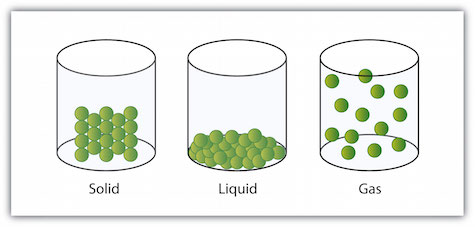
\includegraphics{res/matter_comp.jpg}
  \caption{The change in particle layouts between different states of matter.}
\end{figure}

\begin{description}
  \item[Solids] attractions are stronger than the motion, producing a small
    degree of vibration between the molecules.
  \item[Liquid] the kinetic energy is relatively equal to the attraction
    \begin{itemize}
      \item Translational motion - particles can move or "slide" past other
        particles
    \end{itemize}
  \item[Gas] more kinetic energy than attraction.
\end{description}

Ideal gas is an imaginary gas that perfectly fits all of the assumptions of the
kinetic molecular theory:

\subsection{Theory}
\begin{enumerate}
  \item Gases consist of large numbers of tiny particles that are far apart
    relative to their size.
  \item Collisions between gas particles and between particles container walls
    are elastic collisions.
  \item Gas particles are in continuous, rapid, random motion.
  \item There are no forces of attraction or repulsion between gas particles.
  \item The average kinetic energy of gas partilces depend on the temperature of
    the gas
\end{enumerate}

\subsection{Properties}
Gases usually take up a volume nearly 1-thousand times greater than the volumeof
the corresponding liquid.

\begin{description}
  \item[Elasic collision] a collision in which there is no net loss of kinetic
    energy
    \begin{itemize}
      \item Energy can be transferred, but the total energy of the system
        remains the same
    \end{itemize}
\end{description}

Gases have a low density and cannot be compressed.  However, if you do compress
them, they will just turn into a liquid.  The average kinetic energy of gases
depend on the greatest velocity of the particles.

As the temperature increases, so does the kinetic increase, and vice-versa.  Two
gases at the same temperature will have the same kineitc energy, yet they may
have different average velocity.

Kinetic energy is based upon two factors.  It is expressed as
$1/2(mass)(velocity)^2$

\section{Nature of Gases}
\begin{description}
  \item[Expansion] no define shape or defnite volume (it will fill any enclosed
    container)
  \item[Fluidity] gases flow due to molecular diffusion
  \item[Low density] gases contain very few particles within a definite volume
  \item[Compressibiity] gas particles are pressed close to each other, and can
    get a large amount of gas in a relatively small size
  \item[Diffusion] gas particles spontaneously mix due to their random motion
  \item[Effusion] process via which gas particles pass through a small opening
\end{description}

\section{Gas Laws}
\begin{description}
  \item[Boyle's Law] states that the volume of a fixed mass of gas varries
    inversely with the pressure at a constant temperature.
  \item[Charles's Law] states that volume and temperature are related to each
    other.  If you increase the temperatire that the volume is occupied by the
    gas will also increase.  \textit{(i.e., double the pressure $\rightarrow$
    double the volume)}
\end{description}
